\documentclass[10pt]{article}


% Tous les packages prédéfinis
\usepackage{introLatex}
\usepackage{headfootLatex}
\usepackage{shortcutLatex}
\usepackage{envLatex}
\graphicspath{{logos/}{figures/}}


\begin{document}


% Titre du document
\begin{center}
\textbf{\Large Méthode multipole rapide pour un nuage de points}\\
\vspace*{4pt}
Gaétan Facchinetti \\
{\small 5 décembre 2016\\
\vspace*{5pt}
\textit{Université Paris-Saclay}, \textit{Ecole Normale Supérieure de Cachan}}, \\
\textit{Ecole Nationale Supérieure des Techniques Avancées}\\
\end{center}

\vspace*{22pt}


\begin{multicols}{2}



\section*{Question 1}

Nous avons créer une fonction permettant de renvoyer, pour une densité de point par longueur d'ondre $n_\lambda$ et une fréquence $f$ donnée, un tableau de coordonnées de l'ensemble des points du nuages ainsi que le nombre de $N$ points. Dans notre code ce nombre de points se calcule en fonction des paramètres par la formule, 

\begin{equation}
N = 4s_a(s_b-1) + 2(s_b-2)^{2}
\label{eq:N}
\end{equation}

Avec $s_a = \mathbb{E}(f n_\lambda L/c)+1$ et $s_b = \mathbb{E}(f n_\lambda l/c)+1$, où $L=1$ (m) et $l=0.5$ (m) sont les dimensions de la boite et $c$ la célérité de l'onde dans le milieu considéré Nous avons alors pu représenter en \refig{Q1} les points de discrétisation.


\begin{figure}[H]
  \begin{center}
  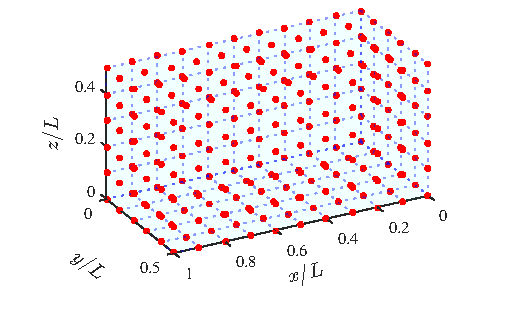
\includegraphics[width=0.95\columnwidth]{Q1_4.pdf}
  \vspace*{-11pt}
  \caption{Points de discrétisation suivant les trois coordonnées spatiales (rouge). $N=252$, $n_\lambda = 10$, $f = c/L$. Pour faciliter la lecture les plans $x=0$, $y=0$ et $z=0$ ont été représentés en cyan.}
  \label{fig:Q1}
  \end{center}
\end{figure}
\vspace*{-22pt}


\vspace*{22pt}



\section*{Question 2}

Notons, pour $i \in \bbrac{1,N}$, $\xv_i$ le vecteur position du point du nuage indicé $i$. Introduisons alors la matrice de la fonction de Green G que nous definissons par : 

\begin{equation}    
\forall (i,j) \in \bbrac{1,N}^{2} \quad G_{i,j} =
 \begin{cases}
   \frac{e^{ik\lb \xv_i - \xv_j \rb}}{\lb \xv_i - \xv_j \rb} & \text{si } i\neq j \\
   1 & \text{si } i=j
 \end{cases}
\end{equation}


Nous notons $\tau_{a}$ le temps d'assemblage de cette matrice. Soit maintenant un vecteur $\rhov$ quelconque de $\R^{N}$. Nous notons $\tau_c$ le temps de calcul du produit matrice vecteur $\Vv = G\rhov$.\\

Nous pouvons remarquer qu'à partir de $N \sim 10 000$ l'assemblade de la matrice est trop gourmand en mémoire et cela rend l'execution sous Matlab impossible. Nous avons donc fait varier $n_\lambda$ à $f$ fixé pour avoir, d'après \refeq{N}, une valeur de $N$ maximale de .... Puis nous avons représenté en \refig{Q2a} et \refig{Q2b} l'évolution de $\tau_a$ et $\tau_c$ en fonction de $N$.



\begin{figure}[H]
  \begin{center}
  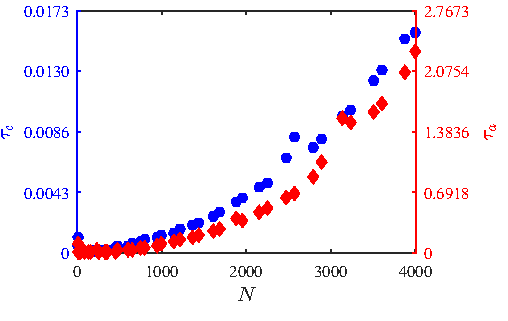
\includegraphics[width=0.95\columnwidth]{Q2a_2.pdf}
  \vspace*{-11pt}
  \caption{Temps d'assemblage de $G$, $\tau_a$ (rouge) et temps de calcul du produit matrice vecteurs $\tau_c$ (bleu) en fonction de $N$. Les deux courbes ont une allure parabolique mais nous pouvons remarquer que, les echelles étant différentes, le temps d'assemblage est plus long}
  \label{fig:Q2a}
  \end{center}
\end{figure}
\vspace*{-22pt}

\begin{figure}[H]
  \begin{center}
  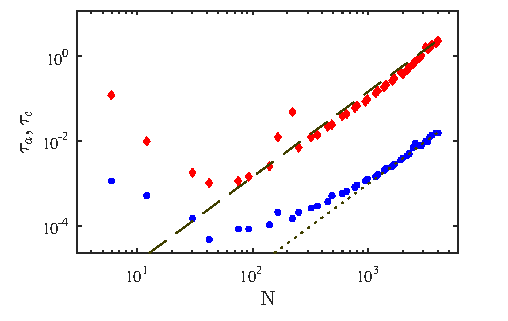
\includegraphics[width=0.95\columnwidth]{Q2b_2.pdf}
  \vspace*{-11pt}
  \caption{Temps d'assemblage de $G$, $\tau_a$ (rouge) et temps de calcul du produit matrice vecteurs $\tau_c$  (bleu) en fonction de $N$. Nous pouvons remarquer ici qu'asymptotiquement $\log(\tau_{a/c}) \simeq 2\log(N)+K_{a/c}$ représentées en pointillé vert avec $K_{a/c}$ constante.}
  \label{fig:Q2b} 
  \end{center}
\end{figure}
\vspace*{-22pt}

Comme il l'est montré en \refig{Q2b}, l'évolution du logarithme de $\tau_a$ avec $N$ tend asymptotiquement vers une droite de pente 2. Il est en cd même pour le logarithme de $\tau_c$ avec $N$. Ceci confirme l'évolution en $O(N^{2})$ du temps d'assemblage et de produit matrice vecteur.



\vspace*{22pt}

\section*{Question 3}

Nous avons calculé la quadrature de Gauss-Legendre à L points en diagonsalisant la matrice tridiagonale définie dans l'énoncé. 

\end{multicols}




\end{document}
